\documentclass[12pt, a4paper]{article}
\usepackage{etex} % расширение классического tex в частности позволяет подгружать гораздо больше пакетов, чем мы и займёмся далее
%%%%%%%%%% Математика %%%%%%%%%%
\usepackage{amsmath,amsfonts,amssymb,amsthm,mathtools} 
%\mathtoolsset{showonlyrefs=true}  % Показывать номера только у тех формул, на которые есть \eqref{} в тексте.

%%%%%%%%%%%%%%%%%%%%%%%% Шрифты %%%%%%%%%%%%%%%%%%%%%%%%%%%%%%%%%
\usepackage{fontspec}         % пакет для подгрузки шрифтов
\setmainfont{Arial}   % задаёт основной шрифт документа
\defaultfontfeatures{Mapping=tex-text}
%why do we need \newfontfamily:
% http://tex.stackexchange.com/questions/91507/
\newfontfamily{\cyrillicfonttt}{Arial}
\newfontfamily{\cyrillicfont}{Arial}
\newfontfamily{\cyrillicfontsf}{Arial}
\usepackage{unicode-math}     % пакет для установки математического шрифта
\setmathfont{Asana Math}      % шрифт для математики
% \setmathfont[math-style=ISO]{Asana Math}
% Можно делать смену начертания с помощью разных стилей



\usepackage{polyglossia}      % Пакет, который позволяет подгружать русские буквы
\setdefaultlanguage{russian}  % Основной язык документа
\setotherlanguage{english}    % Второстепенный язык документа
\usepackage{xcolor}

%%%%%%%%%% Работа с картинками %%%%%%%%%
\usepackage{graphicx}                  % Для вставки рисунков
\usepackage{graphics}
\graphicspath{{images/}{pictures/}}    % можно указать папки с картинками
\usepackage{wrapfig}                   % Обтекание рисунков и таблиц текстом



\usepackage{float}               % возможность позиционировать объекты в нужном месте


%%%%%%%%%% Графика и рисование %%%%%%%%%%
\usepackage{tikz, pgfplots}  % язык для рисования графики из latex'a
\usepackage{amscd}                  %Пакеты для рисования
\usepackage[matrix,arrow,curve]{xy} %комунитативных диаграмм


\DeclareMathOperator{\Var}{Var}
\DeclareMathOperator{\Cov}{Cov}
\def \s{$\sigma$}
\def \xn{$x_1$\ldots $x_n$}
\renewcommand{\labelitemi}{\textcolor{blue}{$\bullet$}}
\renewcommand{\thefigure}{\arabic{section}.\arabic{figure}} 
\newcommand{\zs}{\setcounter{figure}{0}}
%%%%%%%%%% Свои команды %%%%%%%%%%
\usepackage{etoolbox}    % логические операторы для своих макросов
\usepackage{xparse}      % больше команд для создания команд
\begin{document}
\section{Дисперсия и ковариация}
$\Var$
$\Cov$
\section{\s-алгебра}
\s -aлгебра
\section{n $x$-ов}
\xn
\section{другие примеры $x$-ов}
\newcommand{\com}[2]{\ensuremath{x_{#1}} \ldots  \ensuremath{x_{#2}}}
\com{1}{n}\\
\com{a}{z}\\
\com{1}{6}\\ 
\com{(a,b)}{(c,d)}
\section{Список}
\begin{itemize}
\item{несмещенность}
\item{состоятельность}
\end{itemize}
\section{llim}
\newcommand{\llim}[3]{$\lim\limits_{#1 \to #2} #3 $}
\llim{x}{0}{\frac{\sin{x}}{x}}
\section{Номер секции и номер рисунка}
\zs
\begin{figure}[H]
  \centering
    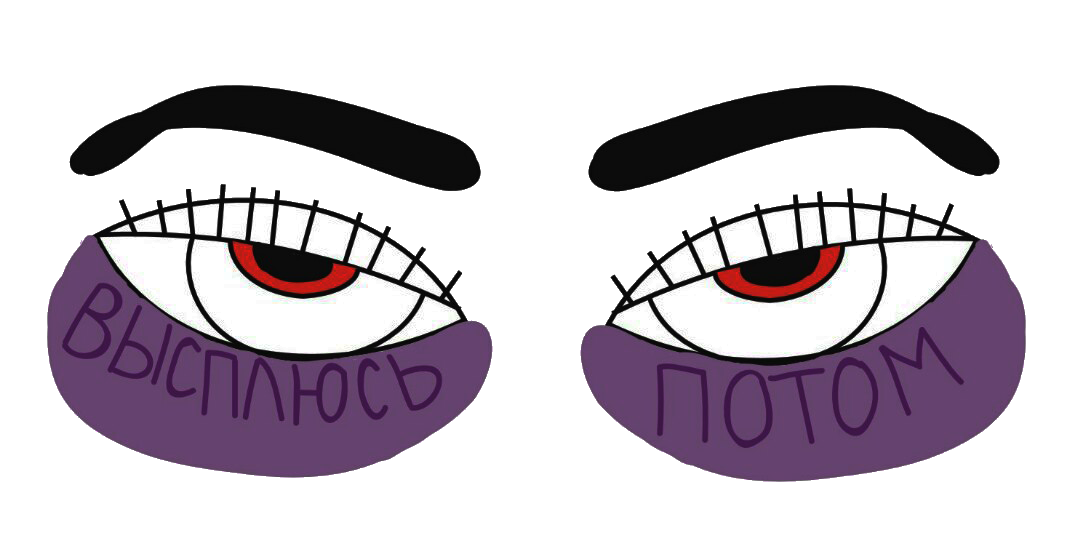
\includegraphics[scale=0.5]{1.png} % replace with image
    \caption{Список с синими точками} 
\end{figure}
\section{Нумерация формул}
\zs
\renewcommand{\theequation}{Eq.(\arabic{equation})} 
\begin{equation} 
\Delta Y_t=\beta_0+\Delta Y_{t-1}+u_t
\end{equation}
\section{Деформация картинки}
\newcommand{\mirro}[1]{\reflectbox{#1}}
\mirro{Сегодня был дождь.}
\newcommand{\updown}[1]{\raisebox{\depth}{\scalebox{1}[-1]{#1}}}
\newline
\updown{Было солнечно 1 августа.}
\section{Важная команда}
\newcommand{\defp}[2]{$\frac{\partial{#1}}{\partial{#2}}$}
\defp{Z}{x}
\end{document}